\documentclass[zavrsnirad]{fer}
% Dodaj opciju upload za generiranje konačne verzije koja se učitava na FERWeb
% Add the option upload to generate the final version which is uploaded to FERWeb


\usepackage{blindtext}
\usepackage{float}

%--- PODACI O RADU / THESIS INFORMATION ----------------------------------------

% Naslov na engleskom jeziku / Title in English
\title{Analysis of basketball training through a mobile application}

% Naslov na hrvatskom jeziku / Title in Croatian
\naslov{Analiza treninga košarke putem mobilne aplikacije}

% Broj rada / Thesis number
\brojrada{1936}

% Autor / Author
\author{Vedran Kumanović}

% Mentor 
\mentor{izv. prof. dr. sc.\@ Matko Orsag}

% Datum rada na engleskom jeziku / Date in English
\date{June, 2025}

% Datum rada na hrvatskom jeziku / Date in Croatian
\datum{lipanj, 2025.}

%-------------------------------------------------------------------------------


\begin{document}


% Naslovnica se automatski generira / Titlepage is automatically generated
\maketitle


%--- ZADATAK / THESIS ASSIGNMENT -----------------------------------------------

% Zadatak se ubacuje iz vanjske datoteke / Thesis assignment is included from external file
% Upiši ime PDF datoteke preuzete s FERWeb-a / Enter the filename of the PDF downloaded from FERWeb
\zadatak{hr_1191247427_73.pdf}


%--- ZAHVALE / ACKNOWLEDGMENT --------------------------------------------------

\begin{zahvale}
  Hvala svima koji su mi pomogli u radu na ovom završnom radu.
  
\end{zahvale}


% Odovud započinje numeriranje stranica / Page numbering starts from here
\mainmatter


% Sadržaj se automatski generira / Table of contents is automatically generated
\tableofcontents


%--- UVOD / INTRODUCTION -------------------------------------------------------
\chapter{Uvod}
\label{pog:uvod}

Osnovni cilj košarkaške igre je stvaranje prilika za poentiranje, pri čemu svi elementi individualne tehnike, timske suradnje i kolektivne taktike nastoje omogučiti igraču da dođe u što povoljniju poziciju za šut. 
Brojna istraživanja pokazala su da učinkovitost šuta, posebice u ključnim trenucima utakmice i s različitih pozicija na terenu, u značajnoj mjeri određuje ishod susreta. 
Primjerice, u analizama utakmica hrvatske lige pokazano je da slobodna bacanja u posljednjih pet minuta čine u prosjeku 42\% poena pobjedničkih ekipa u tijesnim završnicama, u usporedbi s tek 22\% kod poraženih \cite{kumanovic}.
Osim toga, dokazano je da je konačni rezultat utakmice snažno povezan s preciznošću šutiranja s distance, ali i s realizacijom šuteva iz reketa, poput polaganja i zakucavanja \cite{milanovic}.
Bez efikasnog poentiranja, svi ostali tehničko-taktički aspekti igre gube smisao. 
% Ovi elementi igre direktno utječu na ishod utakmice, naglašavajući potrebu za fokusom na tehniku šuta i izbor šuterskih pozicija.

S obzirom na ova saznanja, jasno je da preciznost šuta, kako iz igre tako i s linije slobodnog bacanja, igra presudnu ulogu u konačnom ishodu košarkaških utakmica. 
Intenzivan i ponavljajući samostalni trening neophodan je za napredak u šutu, no mnogim igračima nedostaje mogućnost objektivne analize vlastite tehnike.
Analize šuterske učinkovitosti te biomehanike izvedbe u većini trenažnih procesa još uvijek se uvelike oslanjaju na subjektivne dojmove trenera i ručne statistike.  
Takav pristup često je spor, sklon pogreškama i ne omogućuje dublju, kvantitativnu analizu specifičnih šuterskih situacija, kao što su kut i brzina izbačaja lopte.

Cilj ovog rada je razvoj sustava za automatsku analizu šuterske izvedbe u košarci korištenjem računalnog vida i dubinskih kamera. 
Sustav omogućuje precizno praćenje 3D putanje lopte, detekciju koša te izračun ključnih metrika poput kuta izbačaja, brzine lopte i uspješnosti šuta. 
Takva analiza pruža trenerima i igračima objektivne informacije potrebne za optimizaciju trenažnog procesa i povećanje učinkovitosti.

Za detekciju lopte i obruča koristi se YOLO model treniran na vlastitom skupu podataka, dok se 3D pozicije objekata dobivaju kombiniranjem 2D koordinata s dubinskim informacijama. 
Razvijeni sustav predstavlja korak prema modernizaciji trenažnog procesa u košarci, omogućujući preciznu, automatiziranu i pristupačnu analizu šuta, s ciljem poboljšanja individualne izvedbe i ukupne uspješnosti momčadi.

%---TEORIJSKA PODLOGA I DOSADAŠNJA ISTRAŽIVANJA / THEORETICAL BACKGROUND AND PREVIOUS RESEARCH -----------------------------
\chapter{Teorijska podloga i dosadašnja istraživanja}
\label{pog:teorijska_podloga_i_dosadasnja_istrazivanja}

\section{Umjetne neuronske mreže}
\label{pog:kosarkaska_tehnika_suta}
Duboko učenje temelji se na sposobnosti neuronskih mreža da aproksimiraju složene nelinearne funkcije, što omogućuje njihovu primjenu u širokom spektru problema \cite{Goodfellow-et-al-2016}. 
Ključni model koji se koristi za tu svrhu je višeslojni perceptron (eng. multilayer perceptron (MLP)), koji kroz višeslojne arhitekture modelira odnose između ulaza i željenih izlaza.

Za uspješno treniranje takvih mreža nužno je koristiti tehnike poput regularizacije (za sprječavanje prenaučenosti) i optimizacijskih algoritama (poput varijanti gradijentnog spusta). 
Kada se modeli primjenjuju na velike ulaze, primjerice slike visoke rezolucije ili vremenske nizove, koriste se specijalizirane arhitekture:
\begin{itemize}
  \item \textbf{Konvolucijske neuronske mreže (CNN)} – dizajnirane za obradu vizualnih podataka, koriste konvolucijske slojeve za automatsko prepoznavanje značajki u slikama.
  \item \textbf{Rekurentne neuronske mreže (RNN)} – koriste se za sekvencijalne podatke, poput teksta ili vremenskih nizova, jer mogu modelirati vremensku ovisnost između podataka.
\end{itemize}

Ove arhitekture čine temelj za mnoge praktične primjene dubokog učenja, uključujući analizu videozapisa, detekciju objekata i biomehaničku analizu pokreta, što je izravno povezano s temom ovog rada.

\subsection{Višeslojni perceptron}
\label{pog:viseslojni_perceptron}
Duboke unaprijedne mreže (eng. deep feedforward networks), poznate i kao višeslojni perceptroni (MLP – Multilayer Perceptrons), predstavljaju jedan od najvažnijih modela dubokog učenja. 
Njihov osnovni cilj je aproksimacija nepoznate funkcije \textit{f*}, koja opisuje odnos između ulaznih podataka x i željenog izlaza y, odnosno y=f*(x). 
Riječ je o vrsti umjetne neuronske mreže sastavljene od niza slojeva međusobno povezanih neuronskih jedinica (perceptrona) \ref{fig:mlp}. 
Ove mreže nazivamo unaprijednim jer se informacije kroz mrežu kreću samo u jednom smjeru, od ulaza prema izlazu, kroz niz skrivenih slojeva i nelinearnih transformacija. 
Nema povratnih veza između slojeva, za razliku od rekurentnih neuronskih mreža (RNN), kod kojih izlazi mogu ponovno ulaziti u mrežu i time modelirati vremensku ovisnost \cite{Goodfellow-et-al-2016}.
\begin{figure}[H]
  \centering
  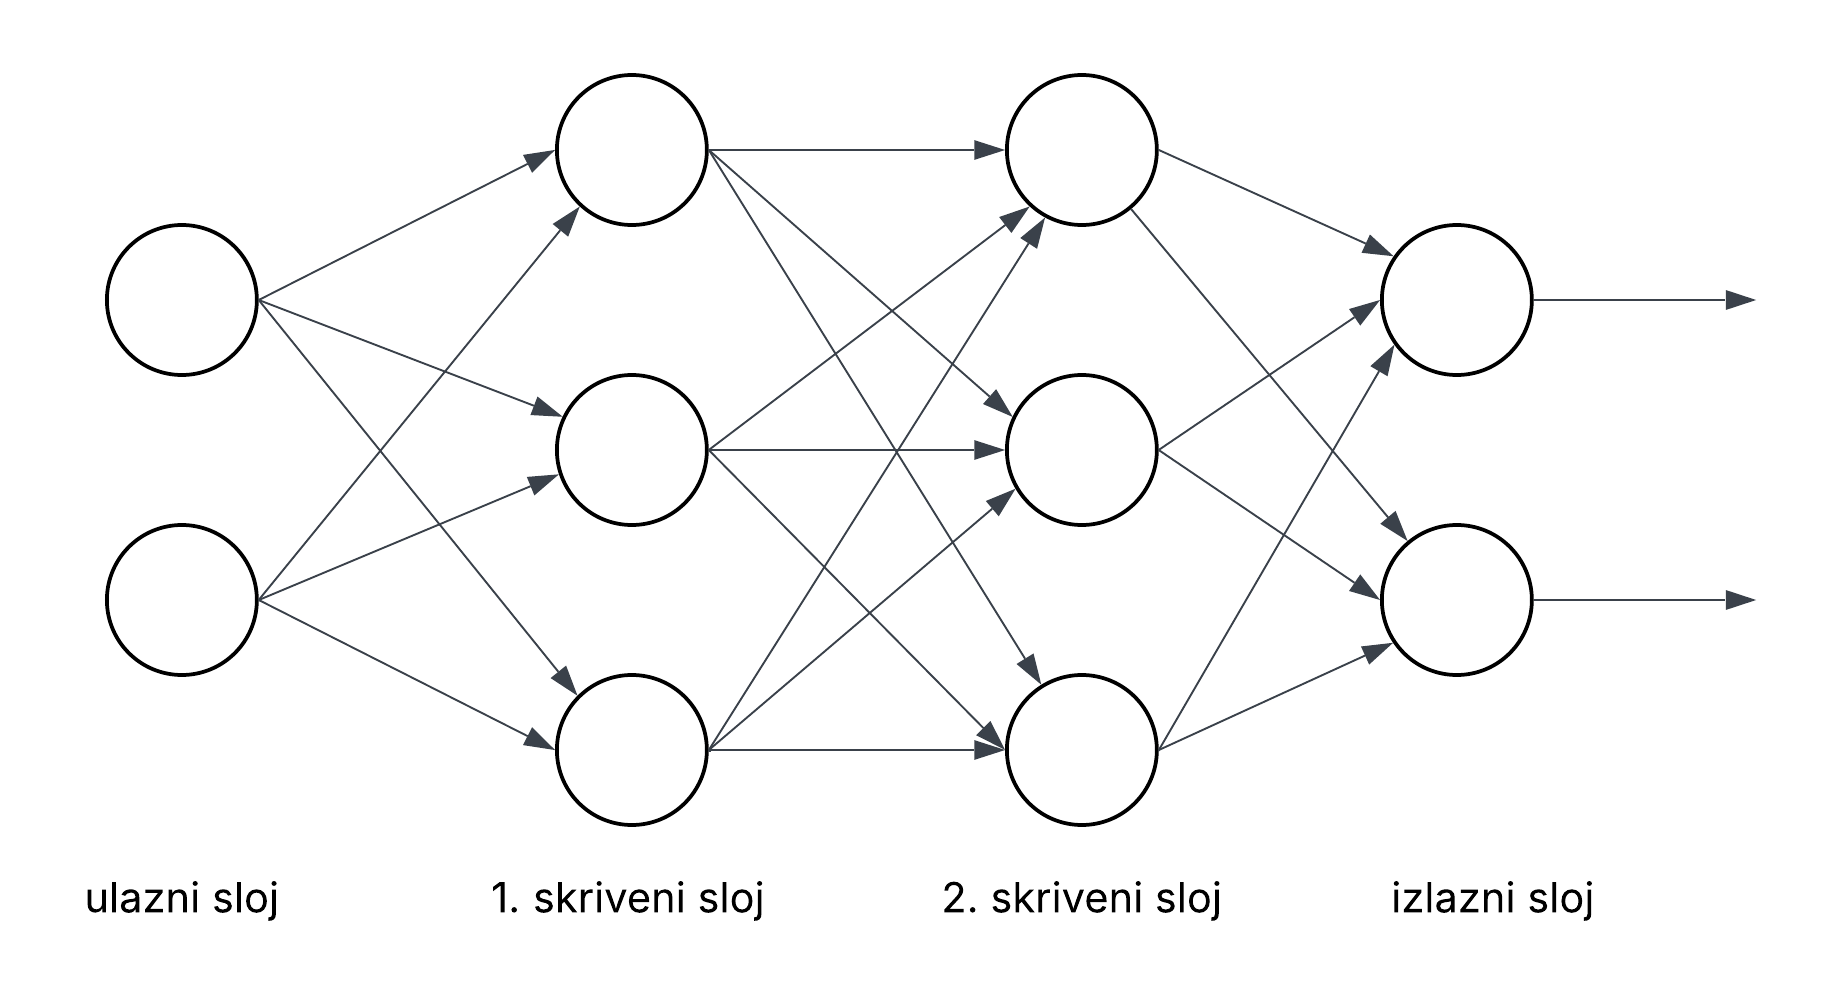
\includegraphics[width=0.6\linewidth]{Figures/mlp.png}
  \caption{Unaprijedna slojevita neuronska mreža 2 × 3 × 3 × 2 \cite{prezentacijaMLP}}
  \label{fig:mlp}
\end{figure}
Da bismo povećali ekspresivnost mreže i omogućili joj modeliranje nelinearnih odnosa, korišteni neuroni moraju imati prijenosne funkcije koje su nelinearne.
U unaprijednim neuronskim mrežama do nedavno je bilo uobičajeno koristiti sigmoidalne prijenosne funkcije, dok se danas se za to preferira uporaba ReLU jer omogućava treniranje dubljih mreža (s većim brojem slojeva) \cite{dalbelo2020neuronske}.

Treniranje MLP mreže provodi se metodom nadziranog učenja, gdje je poznat skup ulazno-izlaznih parova. 
Učenje neuronskih mreža provodi se pomoću postupka propagacije pogreške unatrag (engl. Error Backpropagation), koji omogućuje učinkovit izračun svih parcijalnih derivacija te njihovu primjenu pri određivanju veličine korekcije svake od težina u mreži \cite{dalbelo2020neuronske}.


\subsection{Konvolucijske neuronske mreže}
\label{pog:konvolucijske_neuronske_mreze}
Konvolucijske neuronske mreže (eng. Convolutional Neural Networks - CNN) specijalizirane su vrste neuronskih mreža za obradu podataka koje imaju topologiju nalik na rešetku. 
Za razliku od višeslojnih perceptrona, gdje su svi neuroni u sloju povezani sa svim neuronima u prethodnom sloju, CNN koristi lokalne veze i dijeljenje težina, čime se značajno smanjuje broj parametara i bolje iskorištava prostorna struktura podataka \cite{Goodfellow-et-al-2016}.
\begin{figure}[H]
  \centering
  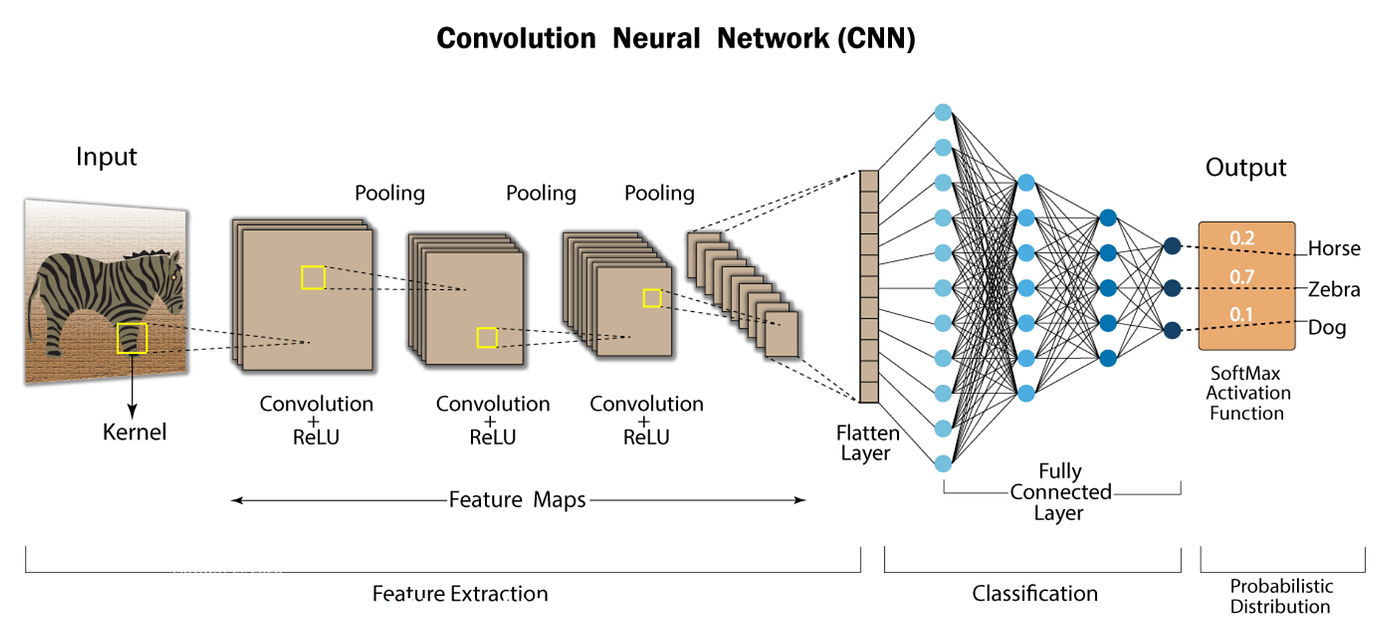
\includegraphics[width=\textwidth]{Figures/cnn_arh.png}
  \caption{Arhitektura konvolucijske neuronske mreže \cite{haque2023cnn}}
  \label{fig:cnn_architecture}
\end{figure}
\noindent Arhitektura CNN-a, prikazana na slici \ref{fig:cnn_architecture}, tipično se sastoji od:
\begin{itemize}
  \item \textbf{Konvolucijskih slojeva} – provode operaciju konvolucije nad slikom, pri čemu se filtar (jezgra, eng. kernel) sustavno primjenjuje na različite dijelove slike kako bi se prepoznali specifični uzorci ili značajke. Ilustrativni primjer konvolucije možemo vidjeti na slici \ref{fig:cnn}. 
Ulazna slika predstavlja kadar iz videozapisa, konvolucijski filtar je matrica vrijednosti koja se pomiče preko slike, a rezultat konvolucije je nova slika koja sadrži informacije o lokalnim značajkama ulazne slike.
  \begin{figure}[H]
    \centering
    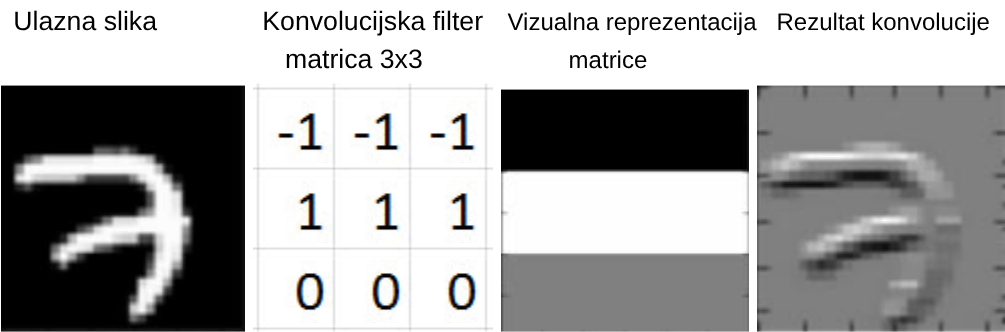
\includegraphics[width=\textwidth]{Figures/convolution.png}
    \caption{Primjer konvolucijske operacije koji prepoznaje rubove, najsvijetliji pikseli označavaju detektirani rub. U ovom slučaju to su gornji horizontalni rubovi \cite{deeplizard_cnn}}
    \label{fig:cnn}
  \end{figure}
  \item \textbf{Slojeva sažimanja (pooling)} – odgovoran je za smanjenje prostorne dimenzionalnosti mapa značajki koje su proizvedene konvolucijskim slojevima (slika \ref{fig:pooling}).
  \begin{figure}[H]
    \centering
    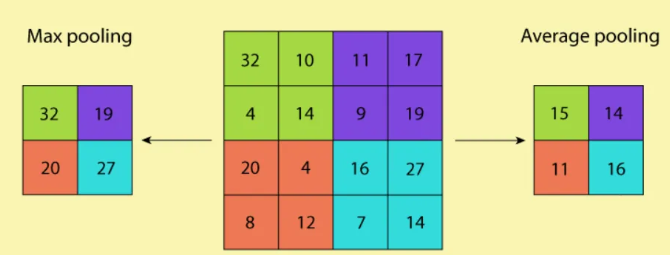
\includegraphics[width=\textwidth]{Figures/pooling.png}
    \caption{Sloj sažimanja, koristi 2 × 2 matricu \cite{haque2023cnn}}
    \label{fig:pooling}
  \end{figure}
  \item \textbf{Aktivacijskih slojeva} – primjenjuje nelinearnu prijenosnu funkciju na izlaz prethodnog sloja, uobičajeno funkcija ReLU opisana formulom \ref{eq:relu}:
  \begin{equation}
    \label{eq:relu}
    ReLU(x) = \max(0, x)
  \end{equation}
  \item \textbf{Potpuno povezanih slojeva} – predstavlja klasični sloj umjetnih neuronskih mreža u kojem je svaki neuron povezan sa svim neuronima prethodnog sloja.
\end{itemize}

Jedna od ključnih prednosti CNN-a je mogućnost hijerarhijskog učenja značajki. 
Početni slojevi otkrivaju osnovne strukture (npr. rubove), dok dublji slojevi uče složenije apstrakcije (npr. oblike lopte, ruku ili koša). 
Upravo zbog toga, CNN modeli su osnova većine modernih sustava za računalni vid, uključujući detekciju objekata, segmentaciju slika i analizu videozapisa.

No ipak, njihova primjena dolazi s određenim izazovima. 
Treniranje zahtijeva značajne računalne resurse i velike količine podataka zbog složene arhitekture i velikog broja parametara. 
Osim toga, modeli su skloni prekomjernom učenju na malim skupovima podataka, a njihova interpretabilnost je ograničena jer je teško uvidjeti koje značajke mreža koristi prilikom donošenja odluka. 
Također, budući da su dizajnirani za podatke rešetkaste strukture, imaju ograničenu sposobnost obrade nepravilnih ili nestrukturiranih oblika.\cite{Goodfellow-et-al-2016,haque2023cnn}.

\section{Detekcija objekata}
\label{pog:detekcija}
Detekcija objekata ključna je zadaća u računalnom vidu koja omogučuje kalsifikaciju i lokalizaciju objekata unutar slike ili videozapisa.
Za razliku od klasifikacije slike, koja određuje prisutnost objekta bez navođenja njegove lokacije, detekcija objekta pruža dodatne informacije o poziciji objekta putem koordinata ograničavajućih okvira (bounding boxes) \cite{v7labs_yolo_2023}.

Metode detekcije objekata mogu se podijeliti u dvije osnovne klase: jednostupanjske (eng. one-stage) i
dvostupanjske (eng. two-stage) metode.
Dvostupanjske metode detekcije najprije izdvajaju potencijalne regije s objektima, a zatim ih naknadno klasificiraju, dok jednostupanjski pristupi istovremeno obavljaju i lokalizaciju i klasifikaciju objekata. 
Glavna razlika između ova dva pristupa očituje se u brzini izvođenja – jednostupanjske metode su znatno brže. 
S druge strane, kada je riječ o preciznosti, obje kategorije postižu usporedive rezultate. 
U nastavku su detaljnije prikazane obje skupine metoda duboke detekcije objekata \cite{nskturad}.

\subsection{Dvostupanjske metode detekcije objekata}
\label{pog:dvostupanjske_metode_detekcije_objekata}
Dvostupanjski pristupi detekciji objekata obavljaju zadatak u više koraka. U prvom koraku, iz ulazne slike se izdvajaju potencijalne regije koje bi mogle sadržavati objekte. 
Nakon toga, za svaku od tih regija provodi se klasifikacija pomoću prethodno naučenog klasifikatora, kojim se regije svrstavaju u odgovarajuće klase objekata. 
Prednost ovih metoda leži u tome što se klasifikacija provodi samo nad ograničenim brojem relevantnih prijedloga, čime se smanjuje utjecaj pozadine i povećava preciznost. 
Među najpoznatijim predstavnicima ovakvog pristupa su RCNN, SPPnet, Fast RCNN i Faster RCNN. 
RCNN modeli proširuju standardne konvolucijske mreže za potrebe detekcije i lokalizacije objekata, pri čemu kao izlaz daju skup bounding boxova za svaki detektirani objekt zajedno s pripadajućom klasom \cite{v7labs_yolo_2023, nskturad}.

\subsection{Jednostupanjske metode detekcije objekata}
\label{pog:jednostupanjske_metode_detekcije_objekata}
Jednostupanjski algoritmi za detekciju objekata analiziraju cijelu sliku u jednom prolazu kroz mrežu te istovremeno predviđaju prisutnost i lokaciju objekata. 
Ovakav pristup značajno je učinkovit u pogledu računalnih resursa i brzine izvođenja, što ga čini pogodnim za primjenu u sustavima s ograničenim hardverskim kapacitetima i u stvarnom vremenu.
Najpoznatije metode ovog tipa su: OverFeat, SSD, YOLO i RetinaNet.

Jedan od najpoznatijih predstavnika ove skupine i model koju ćemo mi koristiti je YOLO, koji koristi potpuno konvolucijsku neuronsku mrežu za istovremenu detekciju svih objekata na slici \cite{v7labs_yolo_2023}. 
YOLO algoritam kao ulaz uzima cijelu sliku i koristi jednostavnu duboku konvolucijsku neuronsku mrežu za detekciju objekata.
Struktura mreže temeljena je na CNN arhitekturi, koja se sastoji od konvolucijskih slojeva, slojeva sažimanja i potpuno povezanih slojeva (slika \ref{fig:yolo_architecture}).
\begin{figure}[H]
  \centering
  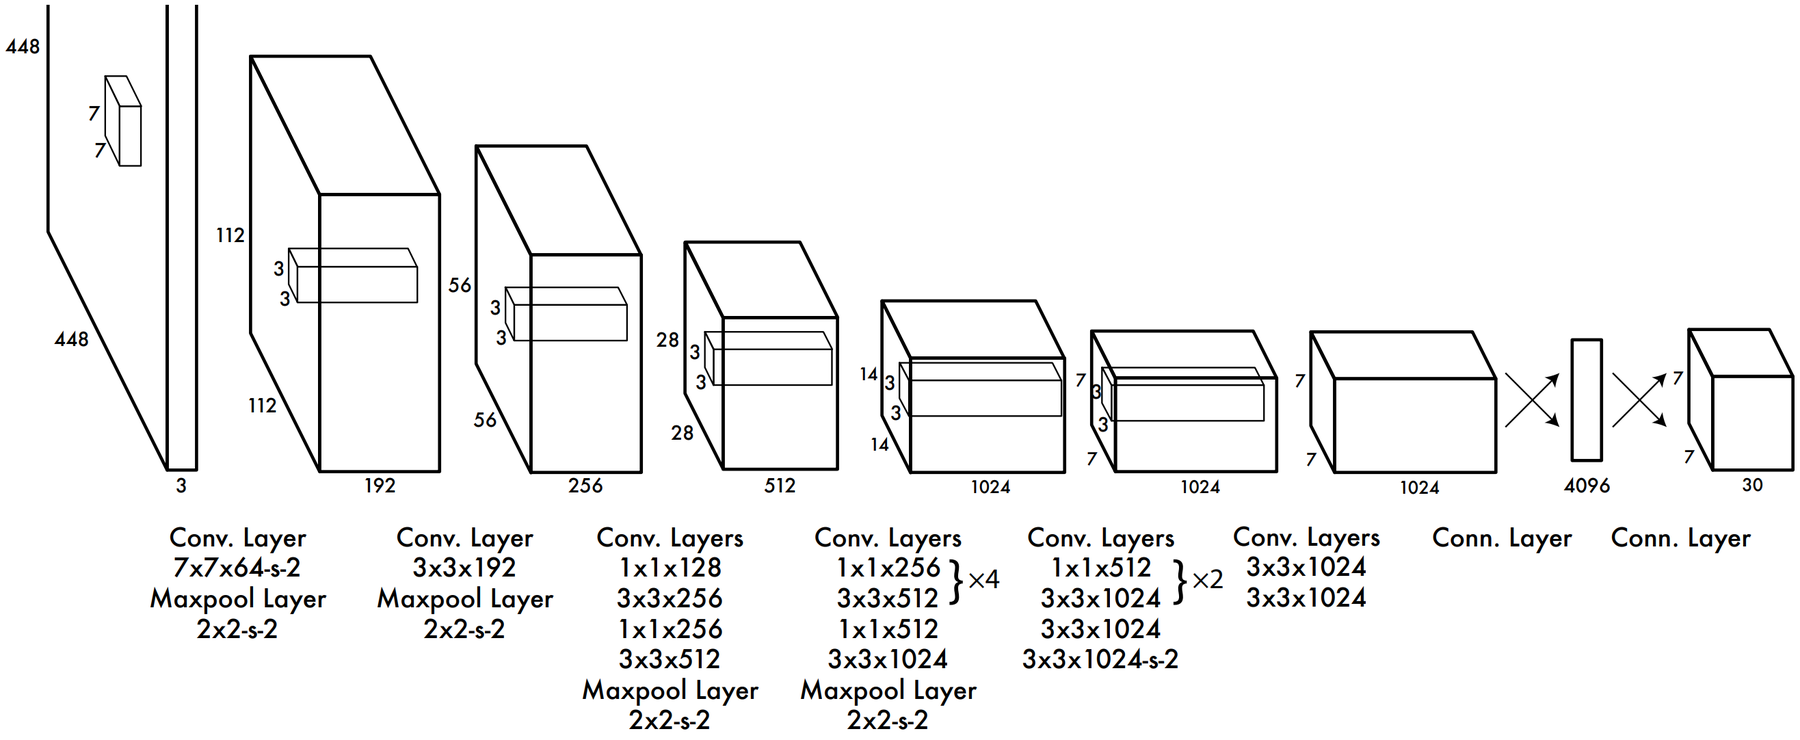
\includegraphics[width=\linewidth]{Figures/Tiny_yolo_architechture.png}
  \caption{Arhitektura CNN modela koji jetemelj za YOLO \cite{v7labs_yolo_2023}}
  \label{fig:yolo_architecture}
\end{figure}
YOLO model dijeli ulaznu sliku na mrežu ćelija, pri čemu svaka ćelija predviđa određeni broj bounding boxova i pripadajućih vjerojatnosti za prisutnost objekta \cite{yolov3}.
Svaka ćelija odgovorna je za detekciju objekata čiji centar leži unutar njezine granice.
YOLO model koristi konvolucijske slojeve za ekstrakciju značajki iz slike, a zatim koristi potpuno povezane slojeve za generiranje predikcija\cite{v7labs_yolo_2023}.
Svaki granični okvir ima predviđanja u obliku (x, y, w, h, s) gdje su (x,y) koordinate okvira unutar ćelije, (w,h) dimenzije graničnog okvira, a „s“ je pouzdanost da se objekt nalazi u okviru \cite{nskturad}.

\section{Dosadašnja istraživanja}
\label{pog:dosadasnja_istrazivanja}
Analiza učinkovitosti šuta u košarci predmet je brojnih istraživanja, kako iz tehničko-biomehaničkog, tako i iz tehnološkog aspekta. 
Neki radovi koriste napredne metode računalnog vida i dubokog učenja, dok se drugi oslanjaju na klasične biomehaničke pristupe.

Jedno suvremeno istraživanje temelji se na korištenju predtreniranog Faster R-CNN modela za detekciju lopte i obruča na videozapisima šuterskih pokušaja. 
Uz pomoć image segmentation tehnika i dvije metode aproksimacije parabole (Bounce-Around i SWISAC), analizira se 2D putanja lopte kako bi se izračunao kut izbačaja i predvidjelo hoće li lopta ući u koš. 
Iako model ne može detektirati loptu u trenutku kada prolazi kroz mrežicu zbog zaklonjenosti (occlusion), algoritam nudi predikciju pogotka na temelju projekcije parabole. 
Prednost ovakvog pristupa je mogućnost davanja automatskih povratnih informacija igraču o kutu izbačaja i točnosti šuta, no detekcija u zaklonjenim kadrovima ostaje izazov.
Također, istraživanje ne uključuje 3D rekonstrukciju putanje lopte pa je potrebno postaviti kameru u optimalan položaj, okomito na liniju šuta, kako bi se dobili točni rezultati \cite{10937574}.

Drugi pristup koji se pokazao korisnim za analizu šuta, iako ne koristi računalni vid, jest biomehanički model koji uzima u obzir kut ubačaja lopte u koš, brzinu izbačaja, rotaciju i početnu visinu lopte. 
Slika \ref{fig:forces} ilustrira četiri ključna svojstva sile za lakše razumijevanje biomehaničkih aspekata šuta. 
Istraživanje ističe kako manji kutovi izbačaja dovode do većih odstupanja od idealne putanje i smanjuju vjerojatnost uspješnog pogotka. 
Najveća pogreška ostvaruje se kod ulaznog kuta od 90°, dok se za kutove ispod 50° znatno smanjuje mogućnost pogotka. 
Također navodi kako su brzina izbačaja i kut izbačaja međusobno su povezani, pri čemu udaljenost šuta izravno utječe na brzinu izbačaja, tj. što je šut udaljeniji, to je potrebna veća brzina. 
Udaljenost također neizravno utječe na kut izbačaja, preciznost šuta opada s većom udaljenošću jer i minimalna odstupanja postaju izraženija zbog duljeg vremena leta lopte.
Rad pruža korisne smjernice za optimizaciju tehnike šuta s biomehaničkog aspekta, ali bez tehničke implementacije ili automatizirane analize \cite{article}.
\begin{figure}[H]
  \centering
  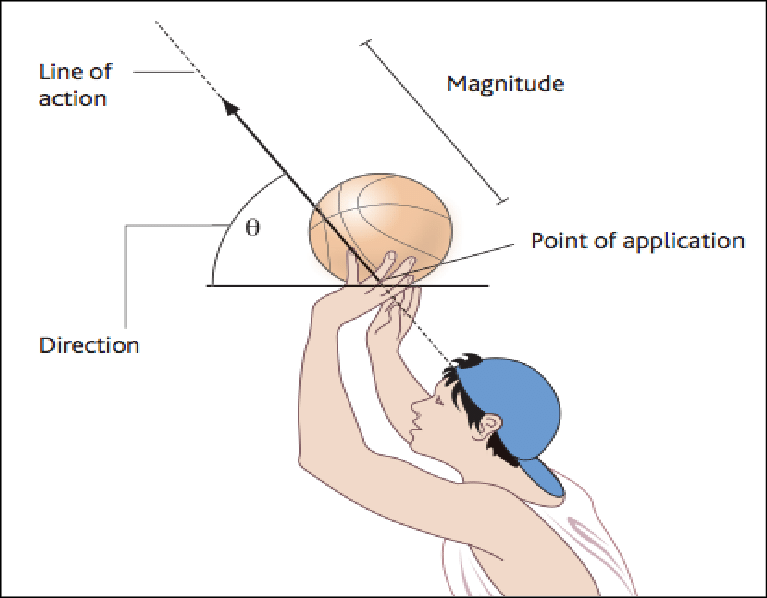
\includegraphics[width=0.6\linewidth]{Figures/The-four-properties-of-force-Hede-Russell-Weatherby-2011.png}
  \caption{Četiri osnovna svojstva sile: iznos (magnituda), smjer djelovanja, točka primjene i pravac djelovanja \cite{article}}
  \label{fig:forces}
\end{figure}
Još jedno istraživanje temeljilo se na teorijskoj analizi, gdje se proučavala putanja lopte prilikom šutiranja slobodnog bacanja.
Analizirao se kut, brzina i rotacija pri ispucavanju. 
Analitički su izračunate kombinacije navedenih parametara koje su rezultirale uspješnim pokušajem.
Optimalni ishod šuta postignut je pri kutu od oko 60° i brzinom od 7,3 m/s \cite{Hamilton1997}.

Sličan pristup primjenjen je u istraživanju \cite{Tran2008}, čiji je cilj bio utvrditi optimalne uvjete otpuštanja lopte pri slobodnom bacanju u muškoj košarci.
Korišteno je stotine tisuća 3D simulacija putanja lopte, pri čemu je analizirano pet varijabli: visina otpuštanja, brzina otpuštanja, kut izbačaja, bočni kut i rotacija lopte.
Pretpostavljeno je da šuter postiže uspješnost od 70\% i da lopta biva otpuštena na visini od 2,134 m.
Rezultati su pokazali da šuter treba lopti dati do 3 Hz rotacije unazad, ciljati prema stražnjem dijelu obruča i izbaciti loptu pod kutom od 52° u odnosu na horizontalu. 
Također, preporučuje se što viši položaj otpuštanja lopte, pod uvjetom da to ne narušava konzistentnost izvođenja šuta.
%---KORIŠTENE TEHNOLOGIJE I ALATI / USED TECHNOLOGIES AND TOOLS -----------------------------
\chapter{Korištene tehnologije i alati}
\label{pog:korištene_tehnologije_i_alati}
U sklopu ovog rada pažljivo su odabrane i implementirane različite tehnologije i alati koji su ključni za razvoj sustava za detekciju i analizu košarkaškog šuta. 

Kao glavni programski jezik korišten je Python, zbog svoje čitljivosti, fleksibilnosti i velike podrške u području računalnog vida i dubokog učenja \cite{python}.
Za dohvat i obradu slike te implementaciju računalnog vida korištena je OpenCV biblioteka. Zahvaljujući svojoj modularnoj strukturi i širokoj podršci u zajednici, OpenCV omogućuje jednostavnu implementaciju zadataka poput obrade slika, filtriranja, praćenja objekata i vizualizacije rezultata \cite{opencv}. 
U sklopu ovog projekta korišten je za obradu video okvira, crtanje bounding boxova, vizualizaciju putanje lopte te manipulaciju slikovnim i dubinskim podacima.
Matplotlib poslužio je za grafički prikaz rezultata, posebno za crtanje i spremanje dijagrama putanje lopte i kuta izbačaja. 

Snimanje videozapisa i dubinskih podataka vršeno je pomoću Oak-D Pro Wide kamere. Ova kamera opremljena je RGB senzorom visoke rezolucije i stereo kamerama za procjenu dubine. 
RGB podatci koristili su se za detekciju objekata, dok su dubinski podaci omogućili rekonstrukciju 3D putanje lopte.
Osim mogućnosti snimanja slike , omogućuje istovremeno izvođenje detekcije objekata na samom uređaju, no taj pristup nije se pokazao dovoljnim, pa je taj dio obavljen na računalu \cite{depthai}.

Za detekciju objekata korištene su novije verzije YOLO modela, unaprijeđene verzija jednoprolaznog detekcijskog algoritma (You Only Look Once), koji omogućuje brzo i precizno prepoznavanje objekata i segmentaciju slike.
YOLO-ov jedinstveni pristup tretira detekciju objekata kao jedan regresijski problem, predviđajući okvire i vjerojatnosti klasa izravno iz slika u jednom prolazu.
YOLO podržava razne zadatke umjetne inteligencije vida kao što su detekcija, segmentacija, procjena položaja, praćenje i klasifikacija.
Njegova najsuvremenija arhitektura osigurava vrhunsku brzinu i točnost, što ga čini prikladnim za različite primjene \cite{ultralytics}.
Za treniranje YOLO modela korišten je Google Colab, online razvojno okruženje koje omogućuje korištenje GPU-a u oblaku. 
Model je treniran na vlastitom skupu podataka snimljenom pomoću OAK-D kamere, a treniranje je provedeno u Colabu zbog jednostavnog pristupa računalnim resursima, lakog rukovanja podacima i brzine izvođenja, čime je omogućena brza iteracija modela i validacija rezultata.




%---RAZVOJ SUSTAVA ZA DETEKCIJU I ANALIZU KOŠARKAŠKOG ŠUTA / DEVELOPMENT OF A SYSTEM FOR DETECTING AND ANALYZING BASKETBALL SHOTS
\chapter{Razvoj sustava za detekciju i analizu košarkaškog šuta}
\label{pog:razvoj_sustava_za_detekciju_i_analizu_kosarkaskog_suta}

\section{Prikupljanje i obrada podataka}
\label{pog:prikupljanje_i_obrada_podataka}

\section{Detekcija objekata korištenjem YOLO modela}
\label{pog:detekcija_objekata_koristenjem_yolo_modela}


\section{Prepoznavanje pokušaja šuta i pogođenih koševa}
\label{pog:prepoznavanje_pokusaja_suta_i_pogodenih_koseva}

\section{Rekonstrukcija 2D i 3D putanje lopte}
\label{pog:rekonstrukcija_2d_i_3d_putanje_lopte}

\section{Određivanje kuta izbačaja i brzine šuta}
\label{pog:odredivanje_kuta_izbacaja_i_brzine_suta}


\section{Mogućnosti prijenosa sustava na mobilne uređaje}
\label{pog:mogucnosti_prijenosa_sustava_na_mobilne_uredaje}


%---REZULTATI I RASPRAVA / RESULTS AND DISCUSSION -----------------------------
\chapter{Rezultati i rasprava}
\label{pog:rezultati_i_rasprava}

\section{Primjeri detekcije i analize šuteva}
\label{pog:primjeri_detekcije_i_analize_suteva}
\section{Evaluacija točnosti detekcije i analize}
\label{pog:evaluacija_tocnosti_detekcije_i_analize}
\subsection{Eksperimenti u kojima se razvijeni postupak dobro ponaša}
\label{pog:eksperimenti_u_kojima_se_razvijeni_postupak_dobro_ponasa}
\subsection{Eksperimenti u kojima postupak nalazi objekte koje nismo tražili (false positive error)}
\label{pog:eksperimenti_u_kojima_postupak_nalazi_objekte_koje_nismo_trazili}

\subsection{Eksperimenti u kojima postupak ne pronalazi tražene objekte (false negative error)}
\label{pog:eksperimenti_u_kojima_postupak_ne_pronalazi_trazene_objekte}


%--- ZAKLJUČAK / CONCLUSION ----------------------------------------------------
\chapter{Zaključak}
\label{pog:zakljucak}

\blindtext


%--- LITERATURA / REFERENCES ---------------------------------------------------

% Literatura se automatski generira iz zadane .bib datoteke / References are automatically generated from the supplied .bib file
% Upiši ime BibTeX datoteke bez .bib nastavka / Enter the name of the BibTeX file without .bib extension
\bibliography{literatura}



%--- SAŽETAK / ABSTRACT --------------------------------------------------------

% Sažetak na hrvatskom
\begin{sazetak}
  Unesite sažetak na hrvatskom.

  \blindtext
\end{sazetak}

\begin{kljucnerijeci}
  prva ključna riječ; druga ključna riječ; treća ključna riječ
\end{kljucnerijeci}


% Abstract in English
\begin{abstract}
  Enter the abstract in English.
  
  \blindtext 
\end{abstract}

\begin{keywords}
  the first keyword; the second keyword; the third keyword
\end{keywords}

%predlozak

% \begin{figure}[htb]
%   \centering
%   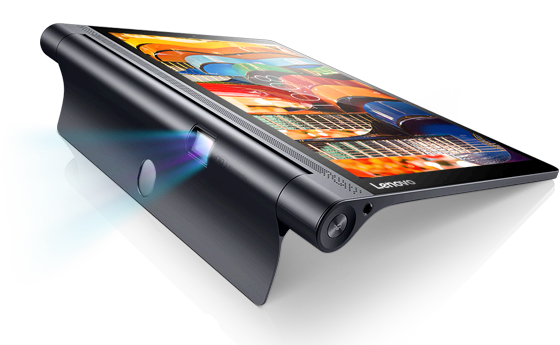
\includegraphics[width=0.38\linewidth]{Figures/lenovo_yoga_tab3_pro_front.png} 
%   \caption{Moja prva slika}
%   \label{slk:prvaslika}
% \end{figure}

% Referenciramo se na sliku \ref{slk:prvaslika} u sredini rečenice, zatim prije zareza \ref{slk:prvaslika}, te zatim na kraju rečenice \ref{slk:prvaslika}.
% Upravo smo testirali radi li naredba \verb|\ref| ispravno u slučaju kada nakon nje slijedi točka.

% Sada slijedi jedna jednadžba:
% \begin{equation}
%   \label{jed:prvajednadzba}
%   \int_{-\infty}^{+\infty}f(t)\,dt=F(\omega)
% \end{equation}
% Jednadžba \eqref{jed:prvajednadzba} je moja prva jednadžba koja defnira par $f(t)\ufrek F(\omega)$ ili $F(\omega)\uvrem f(t)$.

%--- PRIVITCI / APPENDIX -------------------------------------------------------

% Sva poglavlja koja slijede će biti označena slovom i riječi privitak / All following chapters will be denoted with an appendix and a letter
\backmatter

\chapter{The Code}

\Blindtext


\end{document}
